\renewcommand{\fieldheight}{48pt}
\begin{figure}[t]
  \centering
  \begin{tabular}{m{1pt}c@{\hspace{20pt}}m{1pt}c@{\hspace{20pt}}m{1pt}c}
    &\hspace{12pt}\small $t_{40}(\nu=3)$ && \hspace{12pt}\small\texttt{elliptical shell} && \hspace{12pt}\small\texttt{elliptical extreme} \\
    \raisebox{48pt}{\rotatebox{90}{\tiny magnitude $w_i$}} &
    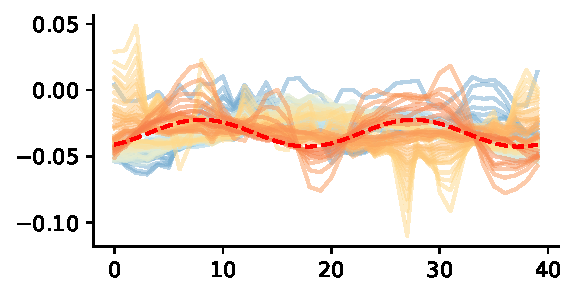
\includegraphics[height=\fieldheight]{rebuttal-figures/elliptical/t3.pdf} &
    \raisebox{48pt}{\rotatebox{90}{\tiny magnitude $w_i$}} &
    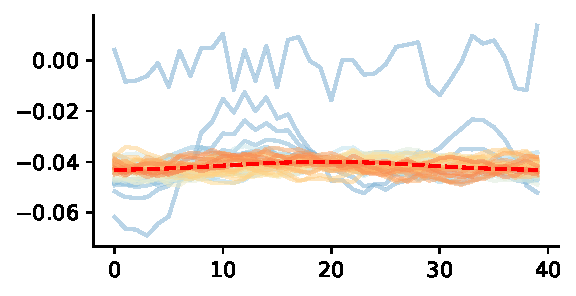
\includegraphics[height=\fieldheight]{rebuttal-figures/elliptical/shell.pdf} &
    \raisebox{48pt}{\rotatebox{90}{\tiny magnitude $w_i$}} &
    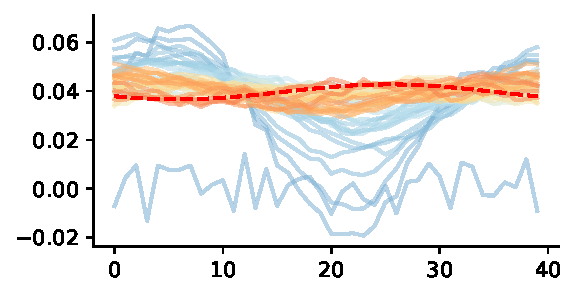
\includegraphics[height=\fieldheight]{rebuttal-figures/elliptical/extreme.pdf} \\
    \noalign{\vskip -40pt}
    &
    \hspace{12pt}\tiny dimension $i$ of weight $\mathbf{w}$ & &
    \hspace{12pt}\tiny dimension $i$ of weight $\mathbf{w}$ &&
    \hspace{12pt}\tiny dimension $i$ of weight $\mathbf{w}$
  \end{tabular}
  \caption{
    单神经元模型 (\labelcref{item:single-neuron-model}) 学习的感受野的演化,以及当在三种椭圆分布的数据上训练时,拟合到最终状态的正弦波(红色虚线):$t_{40}(\nu=3)$ (\textbf{左图}),椭圆表面 (\textbf{中图}),以及一个自定义的椭圆分布,其质量位于椭圆的外侧 (\textbf{右图})。
    在所有情况下,学习到的感受野都是振荡的(正弦波),正如命题 \ref{thm:elliptical} 所预测的。
    拟合的振荡权重与经验感受野之间的 $\ell_2$ 距离,作为经验感受野的 $\ell_2$ 范数的比率分别为(左图)9.77\%,(中图)3.75\%,(右图)4.14\%。
    \emph{参见 \cref{sec:elliptical-experiments} 以获取详细说明。}
}
    \label{fig:elliptical}
\end{figure}
